\begin{blocksection}
\question Draw the environment diagram that results from running the following code.

\begin{lstlisting}
def funny(joke):
    hoax = joke + 1
    return funny(hoax)

def sad(joke):
    hoax = joke - 1
    return hoax + hoax

funny, sad = sad, funny
result = funny(sad(2))
\end{lstlisting}
\begin{solution}[2in]
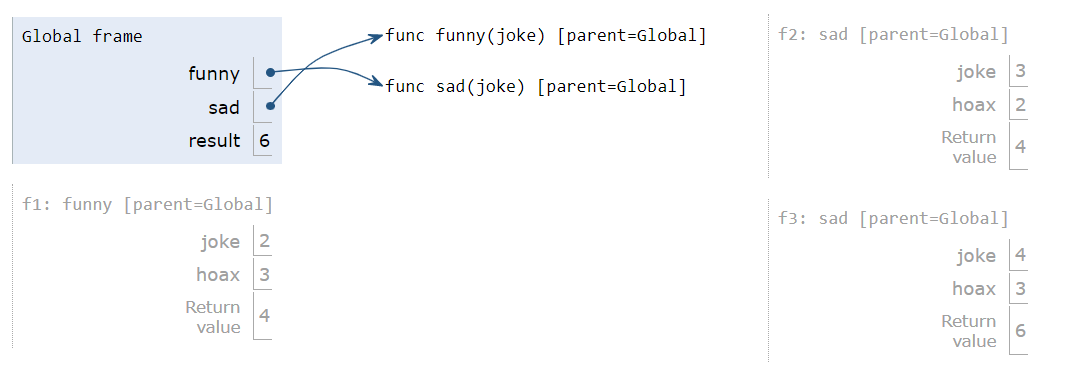
\includegraphics[scale=0.5]{joke.png}
\\
\url{https://tinyurl.com/y5lc4fez}
\end{solution}
\end{blocksection}

\begin{questionmeta}
  The primary purpose of this problem is to teach variable lookup rules and the difference between intrinsic and bound names of functions. 

  Make sure that the students understand how Python looks for a value of a variable, from local (to parent(s)) to global.

  As a reminder, the intrinsic name of a function is the name that belongs to a particular function object. (For a function \lstinline{f}, this name can be accessed and changed through \lstinline{f.__name__}, though telling your students this might just confuse them.) For user defined functions, this intrinsic name is the name used in the \lstinline{def} statement (lambda functions have no intrinsic name). Functions cannot necessarily be referred to by their intrinsic names in code. Because it is associated with the function object, the intrinsic name appear on the right-hand side of an environment diagram, in the "objects" column. 
  
  The bound name(s) of a function, on the other hand, are the names of variables that point to the function object. A function can have many bound names, and the bound names of a function can often change. 
  
  An analogy I like to use for teaching this is beanie babies. Beanie babies come with a little tag attached that gives the canonical name of the plushie, but most people come up with their own names for their beanie babies and largely ignore this name. For example, when I acquired a beanie baby bear, its tag name was ``Glory'', but I called it ``Aces''. The previous owner called it ``Washington''. Depending on the context, different people can call the bear different things, but the name on the tag, which is physically attached to the bear, does not change. Similarly, different frames can have different bound names for a function, but the intrinsic name is attached to the function object and has permanence. 

  When teaching this problem, also remember to evaluate the functions on the RHS first, then assign to variables on the LHS.
\end{questionmeta}
    